% This is samplepaper.tex, a sample chapter demonstrating the
% LLNCS macro package for Springer Computer Science proceedings;
% Version 2.20 of 2017/10/04
%
\documentclass[runningheads]{llncs}
%
\usepackage{graphicx}
%\usepackage[numbers,sort&compress]{natbib}
%\renewcommand\bibname{References}
%https://tex.stackexchange.com/questions/359355/lncs-bibliography-format
\usepackage[%
  square,        % for square brackets
  comma,         % use commas as separators
  numbers,       % for numerical citations;
%  sort,          % orders multiple citations into the sequence in which they appear in the list of references;
  sort&compress, % as sort but in addition multiple numerical citations
                 % are compressed if possible (as 3-6, 15);
]{natbib}
% In the bibliography, references have to be formatted as 1., 2., ... not [1], [2], ...
\renewcommand{\bibnumfmt}[1]{#1.}
\renewcommand{\bibsection}{\section*{References}}

\usepackage[margin=1in,footskip=0.25in]{geometry}
% Used for displaying a sample figure. If possible, figure files should
% be included in EPS format.
%
% If you use the hyperref package, please uncomment the following line
% to display URLs in blue roman font according to Springer's eBook style:
% \renewcommand\UrlFont{\color{blue}\rmfamily}
\newcommand{\toolname}{FuncyTuner\space}


\begin{document}
%
\title{FuncyTuner: Auto-tuning Scientific Applications With Per-loop Compilation}
%
%\titlerunning{Abbreviated paper title}
% If the paper title is too long for the running head, you can set
% an abbreviated paper title here
%
\author{Tao Wang\inst{1} \and
Nikhil Jain\inst{2} \and
David Beckingsale\inst{2} \and
David Boehme\inst{2} \and
Frank Mueller\inst{1} \and
Todd Gamblin\inst{2}}
%
\authorrunning{Tao Wang et al.}
% First names are abbreviated in the running head.
% If there are more than two authors, 'et al.' is used.
%
\institute{Department of Computer Science, North Carolina State University, USA \\
\email{\{twang15, fmuelle\}@ncsu.edu}\\
\and
Lawrence Livermore National Laboratory\\
\email{\{jain6,beckingsale1,boehme3,gamblin2\}@llnl.gov}}
%
\maketitle              % typeset the header of the contribution
%
\begin{abstract}
The de facto compilation model for production software compiles all
modules of a target program with a single set of compilation flags,
typically \emph{O2} or \emph{O3}. Such a per-program compilation
strategy may yield sub-optimal executables since programs tend to have
multiple hot loops with diverse code structures and can be further
optimized using targeted compilation flags. An alternative to the
per-program compilation model is a per-region compilation model that
assembles an optimized executable by combining the best per-region code variants.

In this paper, we demonstrate that a na\"ive greedy approach to per-region
compilation often degrades performance in comparison to the \emph{O3} baseline.
To overcome this problem, we contribute a novel per-loop compilation framework,
\toolname, which employs light-weight profiling to collect per-loop
timing information, and then utilizes a space-focusing technique to construct a
performant executable. Experimental results show that \toolname can reliably
improve performance of modern scientific applications on several
multi-core architectures by 10.3\% and 5.6\% (geometric mean) in
comparison to the \emph{O3} baseline and prior work, respectively.


\keywords{auto-tuning \and per-loop compilation 
\and fine-grained profiling
\and machine-learning \and ICC}
\end{abstract}
%
%
%
\vspace{-2ex}
\section{Introduction}
In the de facto traditional compilation model, all source files of a program are
compiled with a single set of compiler flags, typically O2 or O3.
However, it is well-known that O2/O3 may not generate the most
performant executables~\cite{Chen:2010:EIO:1806596.1806647}. This is
because optimizations enabled by flags such as O2/O3 are empirically
determined to maximize performance for certain benchmark suites, while
other programs and architectural platforms may have different
characteristics that require other optimizations.  As a result, for a
given program, several other compiler flag combinations may exist that
can produce more performant executables than the default O2/O3 choice.

In order to identify the most suitable optimizations for a program,
researchers have proposed several iterative compilation
techniques~\cite{iterativecompilation,1191546,1611551}, such as
compiler flag selection~\cite{Chen:2010:EIO:1806596.1806647,Cavazos:2007:RSG:1251974.1252540,Vaswani:2007:MSE:1251974.1252536}
and phase ordering construction~\cite{Kulkarni:2004:FSE:996841.996863,Nobre:2016:GIC:2907950.2907959,6662511}.  Given a program, iterative
compilation first generates code variants by compiling the source code
with different compiler flags, and then evaluates their performance
either by execution~\cite{1611551,Chen:2010:EIO:1806596.1806647} or
prediction~\cite{Cavazos:2007:RSG:1251974.1252540,cere}.

% their limitations: search algorithm(greedy) and model construction (machine learning), granularity consideration.
%auto-tuning is a more general term than compiler flag selection and phase-ordering.
Several search-based algorithms have been proposed for generating
compiler flag combinations to create code variants, e.g. predictive machine
learning models~\cite{Cavazos:2007:RSG:1251974.1252540} and
optimization flag correlation-based combined elimination
\cite{1611551}, both of which treat random search
\cite{Chen:2010:EIO:1806596.1806647,opentuner,1611551} as their
baselines.  However, the effectiveness of these methods is limited.
While machine learning based predictive models
\cite{Cavazos:2007:RSG:1251974.1252540} perform well on small training
datasets, a recent study~\cite{FursinMGL15} \eat{employing
  crowd-sourcing compilation} shows that their prediction accuracy
drops dramatically for large-scale datasets and exhibits close to
random behavior.  This indicates that the success of predictive models
on small training sets cannot be easily generalized.
%, which raises concern of their fundamental validity.

%On the other hand,
%the state-of-the-art search-based algorithm
Combined elimination (CE)~\cite{PanE06, Pan:2008:taco} takes advantage
of interactions among compiler flags to find the best combination.
However, our evaluation of CE, shown in \Cref{fig:ce}, for three benchmarks on
Intel's Broadwell architecture shows minimal performance benefit in
comparison to the O3 baseline for both the GNU C/C++ compiler (GCC
release 5.4.0) and the Intel C/C++ compiler (ICC release 17.0.4).

\begin{figure}
\centering
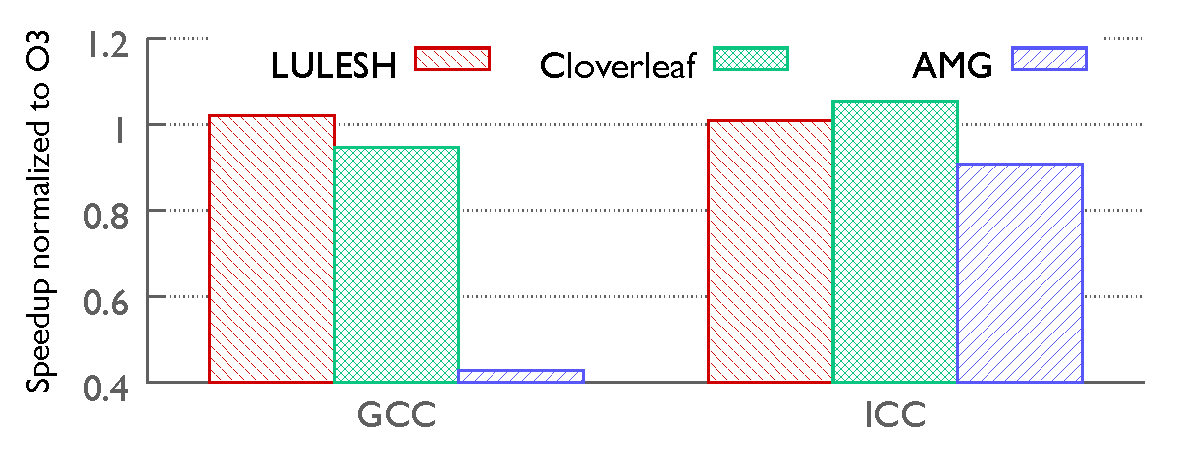
\includegraphics[width=0.7\textwidth]{gnuplot_temp/intro.pdf}
\caption{Combined Elimination does not improve performance significantly.}
\label{fig:ce}
\end{figure}

%
A closer inspection of the experiments for CE revealed that it can
be limited by the results for local minima.  Further, the time
complexity of CE is $O(n^2)$, where $n$ is the number of O3 flags. The
quadratic complexity limits the use of CE for newer GCC versions such
as 5.4.0, which have more than 200 binary optimization flags and 170
multi-valued parameters.  In this work, we address the challenge of
a large search space by employing a novel search space focusing
technique to guide random search.

%In~\cite{PanE06, Pan:2008:taco}, GCC 3.3.3 was evaluated and it has only 38 binary (on/off) options, but it can be much slower for modern GCC, e.g., release 5.4.0, which has more than 200 binary optimization flags and 170 multi-valued parameters.
%In brief, the-state-of-the-art CE is not only time-consuming but also often cannot guarantee performance improvements, as shown in \Cref{fig:ce}.
%coarse-grained random algorithm and fine-grained greedy
%
Fine-grained per-region compilation techniques~\cite{Pan:2008:taco,
  cere, chill, poet} divide a program into different compilation modules and
optimize each separately. 
%
Specifically, source-code level auto-tuners~\cite{chill, poet} focus
on a single simple computation kernel without considering module
interactions in real-world applications. As prior work in compiler flag
selection~\cite{Pan:2008:taco, cere} also assumes that compilation
modules are independent, they assemble an optimized executable by
greedily picking the best code variant of each module. However, the
modules of a program may not be independent due to cross-module
interference, such as shared data structures and link-time
inter-procedural optimizations~\cite{lto, lto2} across multiple
modules.  In particular, link-time optimizations can drive
optimization decisions, such as \emph{loop unrolling}, and may
invalidate earlier transformations that were made independently for
the compilation modules.

{\bf Contributions:}
%
Based on the observations above, we develop a fine-grained auto-tuning
framework, \toolname, that targets modern scientific applications.
%added by Frank
Our overall objective is to extract the best performance out of an
application that is executed repeatedly, such as in high-performance
computing (HPC) where scientists test their hypotheses in experiments
repeatedly with similar inputs using the same algorithms. 
%
To clarify, we {\em neither} attempt to derive a better set of
optimizations for O3, nor do we attempt to generalize a specific set
of optimizations across region boundaries or select different
algorithmic code variants according to input characteristics (in
contract to ~\cite{jiajia,yeom}). Instead, our objective is to 1)
assess whether or not there are module interactions and, if so, 2)
understand how to capitalize on such interactions.

Our target HPC applications exploit multi-core parallelism via OpenMP~\cite{OpenMP}.
Their hot-spots consist of OpenMP loops that account for a significant
fraction of execution time. \toolname outlines these loops and
converts them into individual functions, whose compilation can be
auto-tuned.  To this end, \toolname employs a novel and effective
search space focusing technique to guide random search based
compilation auto-tuning.

%\todo{abstract talks about profiling but not this technique; i think we should say both things in both places.} {changed. Not sure whether it's better.}
%todo{Also, we should mention the search space work earlier when discussing other techniques}{You mean per-region compilation? the advantage is that we want to use it as a direct motivator. If we move it earlier, the transition would be a problem.}
%Our evaluations show that \toolname achieves up to 18.1\% higher
%performance using region-specific optimizations than global O3 flags
%on a set of scientific benchmarks run on several generations of HPC
%architectures.
The contributions of this paper are:
\begin{itemize}
%[leftmargin=6.5mm]
\item We develop a fine-grained per-loop compiler flag selection
  framework, \toolname, that combines program profiling~\cite{caliper}
  % source code transformation, Caliper~\cite{caliper} low-overhead
  % timing infrastructure,
  and search space focusing algorithms to tune hot kernel loops of
  modern scientific programs simultaneously without sacrificing the
  optimization context for production compilers.
  % \todo{too many keywords: also what is source code transformation?
  % i think we can just say light-weight profiling and search space
  % algorithm}
\item We demonstrate that \toolname is able to improve program
  performance for a set of scientific benchmarks by 9.3\% to 10.3\% in
  comparison to the O3 baseline and 4.6\% to 5.6\% relative to prior work,
  both in geometric mean, on several generations of HPC architecture.
%
  %Our \toolname further has the potential to improve machine learning
  %based predictive modeling techniques in the future.
  % \todo{not sure what the potential ML bit is? Can we claim beyond
  % state of the art?} {Previous work show ML never beats random
  % search in terms of program performance improvement}.
\item We conduct an in-depth case study for the Intel compiler tool chain to
  show how fine-grained compiler
  flag selection affects inter-module dependencies and demonstrate
  that it should not be performed greedily, but rather in a focused and targeted manner.
%\todo{is there something specific to Intel? If not, why mention that} {Yes. xiar and xild must be used, and they are not part of ICC}
\end{itemize}

Our \toolname implementation automates these steps, with the
exception of profile instrumentation and collection of timing results,
which are manual in our research prototype, but could be automated
with further engineering effort invested (but are of no research value).

% Paper organization
\iffalse
\todo{I dont think this is useful}
Section \ref{design} first defines terminologies and notations used in this paper, after which \toolname framework and work flow design considerations are explained.
Section \ref{experiment design} gives a brief overview of all experimental settings, such as benchmarks, platforms, and measurement methodology.
The overall tuning results for our benchmark suite are presented in section \ref{results and analysis} to show the effectiveness of \toolname.
Related work is discussed in section \ref{related work}.
Section \ref{conclusion} summarizes this paper and discusses work in detail future work.

iterative compilation~\cite{iterativecompilation, 1191546, 1611551} to search  space of . and auto-tuners~\cite{activeHarmony, opentuner, Zhang:2012:AAS:2259016.2259037}, to take

Motivating example: vectorization or not, to show per-loop compilation may be useful. Can also extract motivation from Peak~\cite{Pan:2008:taco}.

Contribution:

Research questions:
\begin{enumerate}
\item granularity: how to split code
\item stability/sensitivity: R, FR, CFR
\item Effectiveness
\end{enumerate}

Use LULESH as an example for in-depth analysis
\begin{enumerate}
\item why CFR is better than G.realized
\item why CFR is not as good as G.expected
\item Is G.expected a tight upper bound?
\end{enumerate}

Experimental evaluation:
\begin{enumerate}
\item LULESH
\item Cloverleaf
\item AMG
\end{enumerate}

Discussion:

Iterative compilation is a very important compiler-based auto-tuning technology to improve program performance. Search space is too large for exhaustive enumeration. The critical limitation of the state-of-the-art is lack of knowledge of interactions among different compilation flags. It is challenging to automatically derive compiler flag interactions.

Runtime parameter auto-tuning is another effective techniques to improve program performance. Application self-tuning, library auto-tuning, compiler-based code variant tuning. Previous work does not combine iterative compilation and runtime parameter tuning together.

Two possible contributions:
\begin{enumerate}
\item automatically extract compiler flag interactions to reduce space search overhead.
\item combine compile-time and runtime tuning.
\end{enumerate}
\fi


\section{First Section}
\subsection{A Subsection Sample}
Please note that the first paragraph of a section or subsection is
not indented. The first paragraph that follows a table, figure,
equation etc. does not need an indent, either.

Subsequent paragraphs, however, are indented.

\subsubsection{Sample Heading (Third Level)} Only two levels of
headings should be numbered. Lower level headings remain unnumbered;
they are formatted as run-in headings.

\paragraph{Sample Heading (Fourth Level)}
The contribution should contain no more than four levels of
headings. Table~\ref{tab1} gives a summary of all heading levels.

\begin{table}
\caption{Table captions should be placed above the
tables.}\label{tab1}
\begin{tabular}{|l|l|l|}
\hline
Heading level &  Example & Font size and style\\
\hline
Title (centered) &  {\Large\bfseries Lecture Notes} & 14 point, bold\\
1st-level heading &  {\large\bfseries 1 Introduction} & 12 point, bold\\
2nd-level heading & {\bfseries 2.1 Printing Area} & 10 point, bold\\
3rd-level heading & {\bfseries Run-in Heading in Bold.} Text follows & 10 point, bold\\
4th-level heading & {\itshape Lowest Level Heading.} Text follows & 10 point, italic\\
\hline
\end{tabular}
\end{table}


\noindent Displayed equations are centered and set on a separate
line.
\begin{equation}
x + y = z
\end{equation}
Please try to avoid rasterized images for line-art diagrams and
schemas. Whenever possible, use vector graphics instead (see
Fig.~\ref{fig1}).

\begin{figure}
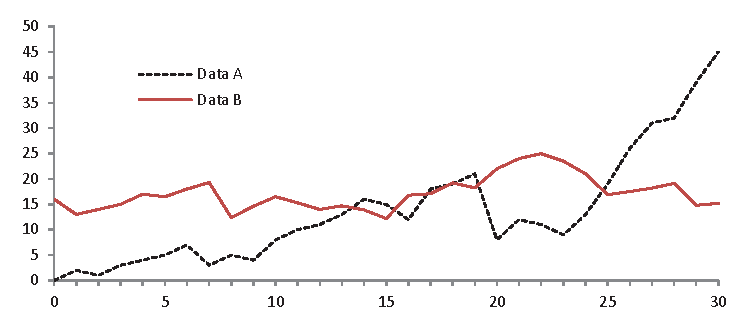
\includegraphics[width=\textwidth]{fig1.eps}
\caption{A figure caption is always placed below the illustration.
Please note that short captions are centered, while long ones are
justified by the macro package automatically.} \label{fig1}
\end{figure}

\if 0
\begin{theorem}
This is a sample theorem. The run-in heading is set in bold, while
the following text appears in italics. Definitions, lemmas,
propositions, and corollaries are styled the same way.
\end{theorem}
%
% the environments 'definition', 'lemma', 'proposition', 'corollary',
% 'remark', and 'example' are defined in the LLNCS documentclass as well.
%
\begin{proof}
Proofs, examples, and remarks have the initial word in italics,
while the following text appears in normal font.
\end{proof}

For citations of references, we prefer the use of square brackets
and consecutive numbers. Citations using labels or the author/year
convention are also acceptable. The following bibliography provides
a sample reference list with entries for journal
articles~\cite{ref_article1}, an LNCS chapter~\cite{ref_lncs1}, a
book~\cite{ref_book1}, proceedings without editors~\cite{ref_proc1},
and a homepage~\cite{ref_url1}. Multiple citations are grouped
\cite{ref_article1,ref_lncs1,ref_book1},
\cite{ref_article1,ref_book1,ref_proc1,ref_url1}.
\fi
%
% ---- Bibliography ----
%
% BibTeX users should specify bibliography style 'splncs04'.
% References will then be sorted and formatted in the correct style.

%\bibliographystyle{splncs04}
\bibliographystyle{splncsnat}
\bibliography{ref.bib}

\if 0
\begin{thebibliography}{8}

\bibitem{ref_article1}
Author, F.: Article title. Journal \textbf{2}(5), 99--110 (2016)

\bibitem{ref_lncs1}
Author, F., Author, S.: Title of a proceedings paper. In: Editor,
F., Editor, S. (eds.) CONFERENCE 2016, LNCS, vol. 9999, pp. 1--13.
Springer, Heidelberg (2016). \doi{10.10007/1234567890}

\bibitem{ref_book1}
Author, F., Author, S., Author, T.: Book title. 2nd edn. Publisher,
Location (1999)

\bibitem{ref_proc1}
Author, A.-B.: Contribution title. In: 9th International Proceedings
on Proceedings, pp. 1--2. Publisher, Location (2010)

\bibitem{ref_url1}
LNCS Homepage, \url{http://www.springer.com/lncs}. Last accessed 4
Oct 2017
\end{thebibliography}
\fi
\end{document}
